\section*{Overview}

The convex hull trick is the optimization I look for when a DP transition has the form
\[
dp[i] = \min_j (m_j x_i + b_j)
\]
or the same expression with \(\max\) instead of \(\min\). Each previous state contributes a line, and answering the
transition means finding the best line at one query point \(x_i\).

\section*{When to Use It}

Use it when:

\begin{itemize}
  \item the transition can be rewritten as evaluating lines \(y = mx + b\),
  \item many candidate lines accumulate over time,
  \item the problem gives monotone slopes, monotone queries, or some other structure that makes line maintenance cheap,
  \item the naive \(O(n^2)\) DP is too slow.
\end{itemize}

If the slope order or query order is arbitrary, a Li Chao tree or a more general line container is often the safer
implementation.

\section*{Core Idea}

Treat each transition source as a line and each target state as a query point.

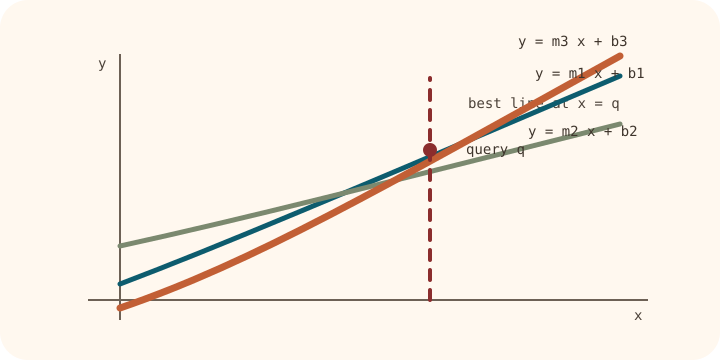
\includegraphics[width=\textwidth]{figures/lower-hull.svg}

For the monotone deque version, I maintain the lower hull of useful lines. When a new line arrives, any older line
that can never again be the minimum gets removed from the back. When queries come in monotone \(x\)-order, I can
also pop from the front while the next line is better at the current \(x\).

That turns a quadratic DP into linear hull maintenance plus one pass of queries.

\section*{Operations}

\begin{itemize}
  \item \textbf{add line}: insert a new line with slope order already guaranteed,
  \item \textbf{remove dominated line}: compare intersections implicitly and pop the middle line if it became useless,
  \item \textbf{query}: while the second line beats the first at the current \(x\), discard the front line.
\end{itemize}

The note code implements the common special case: minimum queries, increasing slopes, increasing query \(x\).

\section*{Correctness Intuition}

On a lower hull, every line that survives owns some interval of \(x\)-values where it is optimal. Those intervals
appear in the same order as the lines on the hull.

When a new line makes the previous intersection order non-monotone, the middle line loses its interval completely and
can be deleted forever. Likewise, once the second line beats the first at the current query \(x\), the first line can
never return as the minimum for any later query because the queries only move rightward.

So both kinds of popping are permanent, which is why the total work stays linear.

\section*{Complexity Analysis}

\begin{itemize}
  \item add line: amortized \(O(1)\),
  \item query: amortized \(O(1)\),
  \item total for \(n\) insertions and \(n\) monotone queries: \(O(n)\),
  \item memory: \(O(n)\).
\end{itemize}

These bounds belong only to the monotone version. General variants are usually \(O(\log n)\) per operation.

\section*{Implementation}

The reference code stores a deque of lines and uses cross multiplication with \texttt{\_\_int128} to avoid precision
bugs in the dominance test. That is deliberate: floating-point intersection code often works until one ugly test case
arrives.

The interface is small:

\begin{itemize}
  \item \texttt{add\_line(m, b)}
  \item \texttt{query(x)}
\end{itemize}

\section*{Common Pitfalls}

\begin{itemize}
  \item Using the monotone deque version when slopes or query points are not monotone.
  \item Mixing up minimum hulls and maximum hulls without flipping the inequalities consistently.
  \item Comparing line intersections with floating point when integer cross multiplication is available.
  \item Forgetting that equal slopes need special handling if both lines are inserted.
  \item Writing the hull correctly but failing to derive \(m\) and \(b\) from the DP transition cleanly.
\end{itemize}

\section*{Practice Problems}

\begin{itemize}
  \item DP recurrences of the form \(dp[i] = \min_j (dp[j] + a_j \cdot x_i + c_j)\).
  \item Problems where the array order already guarantees monotone query points.
  \item Tasks that are almost Li Chao tree problems but become linear after sorting or natural monotonicity.
\end{itemize}

\section*{References}

\begin{itemize}
  \item \href{https://cp-algorithms.com/geometry/convex_hull_trick.html}{cp-algorithms: Convex hull trick and Li Chao tree}.
  \item \href{https://usaco.guide/CPH.pdf}{Competitive Programmer's Handbook}.
  \item \href{https://codeforces.com/catalog}{Codeforces Catalog}.
\end{itemize}
